\chapter{\label{ch:3-mdc_model-reactivation_workflow-instruction_template}Multilevel Dynamic Conservation Model, Reactivation Workflow and Modular Instruction Framework}
In the previous two chapters, we explored the new conservation practices of live media art from two perspectives: from the practical application and outcomes of initiatives and the theoretical and conceptual framework. We examined the developed models for conservation, identifying their common structural elements, and we saw how, conceptually, they strive to apply and consolidate the new conservation paradigms. However, while we can identify similarities between the new conservation practices (particularly in the artwork's acquisition, identification, and iteration), notable differences also emerge.\\
This issue leads us to ask whether it might be possible to discuss standardisation. Standardising conservation practices would have numerous advantages: enhancing accessibility, interoperability, consistency of descriptions, and the efficiency of the tools and systems used. Additionally, they would benefit conservators, who could receive standardised training through specific programs (such as university courses), thereby improving their overall activities and skills. Artists and their collaborators could also adopt standardised procedures and methodologies, improving the conservation of works within their own archives and facilitating acquisitions by third parties. In other words, standardisation could offer significant advantages for the interaction between the various ecosystems involved in the preservation of live media art.\\
Specific standards have already been developed for museum and archive collections, such as \textit{Collection Management Systems} (CMS), also known as \textit{Information Retrieval Systems}. These systems are thought to be integrated into managing and documenting collections, allowing users to search for documents, information within them, and metadata in the databases and their relational structures \cite{dekker2018collecting}. One of the most commonly used CMS in the context of new documentation models is the \textit{Open Archive Information System} (OAIS), which provides guidelines for how archives should acquire, preserve, and ensure the accessibility of digital data over time. OAIS outlines the roles of both the archive and its users, focusing on making preserved information understandable and usable in the future, even if the original technologies become obsolete. However, OAIS and other CMSs are designed to preserve digital data, not specifically for conserving live media artworks. These systems can be integrated into new conservation practices but were not developed specifically for it. On the contrary, live media art conservation models should define how to document, collect, organise, and conserve a work, considering its different components \cite{dekker2018collecting}. Despite numerous attempts, live media art conservation models fail to function as practical standards, often only accepted within the museums or organisations that developed them.\\
\begin{quote}
    "Despite numerous initiatives undertaken during the last two decades, the notion and organisation of artwork-related documentation in museums that collect contemporary art remains neither standardised nor fixed, and, moreover, it is currently facing major challenges" \cite{wielocha2024collections}
\end{quote}
There are many reasons for this lack of standardisation, including the nature of the art itself, the use of cutting-edge technologies and presentation formats, always unique and hard to uniform. Therefore, models developed by institutions are still in their infancy in comparison to the complexity of the art and thus still heavily depend on the museum’s history, subject, scale, and structure \cite{wielocha2024collections}. Moreover, the absence of standardisation stems from the practice of conservation itself, in which the concepts of authenticity and identity that should form the basis of these models are still in development, far from reaching a fully defined, consolidated, and, especially, shared state. Therefore, it may not yet be the time to talk about standardisation—and perhaps it never will be. In this context, the best approach may be to remain heterogeneous and flexible.\\
Given this, we propose addressing the issue from a different perspective, moving beyond the idea of a fixed model or standard and instead using the concept of a meta-model to represent conservation practices. The concept of a meta-model, which emerged in the late 1980s, is now used in various scientific fields, such as mathematics, electronics, and computer science. Suppose we define a model as an abstraction of a real phenomenon. In that case, the meta-model is another abstraction that describes the properties of one or more models—similar to how metadata describes data.
\begin{quote}
“A metamodel is also a model, but its universe of discourse is a set of models, namely those models that are of interest to the creator of the metamodel” \cite{Liu2009-od}.    
\end{quote}
Although we slightly move from the more common definition in computer science, we define the meta-model as a set of abstractions from the models introduced in Chapter~\ref{ch:1-state_of_the_art} and the conservation paradigms in Chapter~\ref{ch:2-new_conservation_paradigms}. Its purpose is to present the properties of a \textit{Creative Work} (artworks, artefacts, projects, etc.) in the context of its conservation. This meta-model serves as a general framework for understanding conservation and can be used to design practical models for preservation, documentation and archiving.\\
In environments like museums, with a team of conservators, such a meta-model can be used to structure a specific model and include details inherent to the institution, such as administrative rules, systems to improve communication with the internal archive, and so on. However, the meta-model can also be applied in smaller contexts, such as organising an artist’s personal computer folders or structuring the repository of an artistic project. Sharing the same organisational structure at a higher (meta) level could make the acquisition process more accessible to museums. A meta-model take into account the network of entities related to the creative works and their relation, promoting a controlled multiplicity of applications. This means having several applications that follow a set of guidelines and can marge into the properties used.\\
So, while we may not achieve full standardisation benefits, a meta-model can simplify the sharing and accessibility of documentation and conservation processes.\\
The meta-model presented in this chapter is the \textit{Multilevel Dynamic Conservation} (MDC) model, developed from the representation of an artwork as a multi-typological archive and as an extension of a model created between 2009 and 2014 at the Centro di Sonologia Computazionale (CSC) at the University of Padua for musical installations. This meta-model is designed to define administrative models for archiving and conserving creative works and their related heterogeneous components and documentation. This chapter will also introduce two other essential tools that can be paired with the MDC model: a workflow for the reactivation process called CATTA (\textit{Collection}, \textit{Assessment}, \textit{Transcription}, \textit{Transmission}, and \textit{Archiving}) and a template for the compilation of the artworks' technical instructions called \textit{Modular Instruction Framework} (MIF). The latter, developed from the instructions used in electronic music scores, also incorporates the adaptation of the Visual Language for describing mappings as defined by Marije Baalman in \cite{baalman2022composing}.\\
All these models summarise the state of the art, considering the most important outcomes of the projects analysed in Chapter~\ref{ch:1-state_of_the_art} and the new conservation paradigms studied in Chapter~\ref{ch:2-new_conservation_paradigms}. The next chapter will demonstrate the MDC model's adaptability across different application contexts. Appendices~\ref{ax:a-michele_sambin_videoloop}, \ref{ax:b-hybrid_reactivation_il_caos_delle_sfere}, \ref{ax:c-the_score_in_live_electronics_music}, and \ref{ax:d-sustainability_and_longevity_of_nimes} will show the CATTA reactivation workflow's applications and the compilation of the instructions.

\section{Multilevel Dynamic Conservation (MDC) Model}
The first version of the \textit{Multilevel Dynamic Conservation} (MDC) Model was developed at the Centro di Sonologia Computazionale (CSC) in 2009 to extend their audio preservation methodology \cite{bressan2016atr, fantozzi2017tape, pretto2019computing}. It was left aside around 2014, but work on the model was revived in January 2021 as part of this PhD research project, with support from both the CSC and Audio Innova Srl\footnote{Audio Innova Srl is a spin-off of the University of Padua, co-founded by Sergio Canazza, who currently serves as both CEO of the company and Director of the CSC. Audio Innova is partner of the PhD research project.}.\\
The CSC is a laboratory at the University of Padua, established in the 1970s, dedicated to research and production in digital sound and computer music \cite{canazza2019four, canazza2022gesture}. Its work ranges from tape music to interactive music installations. Given the large amount of music created on magnetic tapes \cite{pretto2020active}, CSC researchers developed a preservation method specifically for this material, including specific software for supporting the creation of preservation copies of analogue recordings (PSKit) \cite{fantozzi2017tape}. This preservation method is still widely used today by both the CSC and Audio Innova for digitisation projects.\\
However, this methodology still proves inadequate for a significant portion of the CSC's artworks. Since the 1990s, CSC production has gone beyond tape music and included multimedia installations and performances. To preserve these more complex works, CSC researchers began expanding their conservation approach to address the challenges of live media art.\\
Between 2009 and 2014, CSC researchers worked on a series of case studies focused on Carlo De Pirro’s installations in a project called CAPIRE (\textit{CArlo De PIrro: Restoring an Experience}). The project led to the creation of a model for preserving and reactivating interactive multimedia art. As an expansion of their audio preservation strategy, this model introduced new methods for preserving all the elements of interactive multimedia art, as well as the experience it creates \cite{bressan2014challenge}.\\
The multilevel model developed by the CSC is a functional categorisation of documents and is an extension of the CIDOC Conceptual Reference Model (CIDOC-CRM), an ISO standard for describing cultural heritage. The model borrows concepts from both audio preservation and computer science. On the one hand, as an extension of the audio preservation methodology, it incorporates the idea of a preservation copy. The preservation copy is an artefact designed to be stored and maintained as the preservation master \cite{miliano1999iasa}. It consists of an organised dataset containing all the information the original document represents, along with metadata and documentation about the preservation process.\\
On the other hand, the model is structured as a multilevel hierarchy based on a framework for preserving scientific data used in computer science. In this context, the multilevel structure includes \textit{bit} (the lowest level of representation), \textit{data} (attributes), \textit{record} (tuples), and \textit{experience} (the knowledge generated by interpreting the data).\\
In the context of artwork preservation, the preservation copy is defined as follows:
\begin{itemize}
    \item \textit{Bit}: Every part of the original artwork that can be directly preserved, including both digital and physical objects. (The preservation of digital objects follows the general conceptual model defined by the OAIS reference model);
    \item \textit{Data}: Technical notes, comments, and relevant information about the creation of the artwork;
    \item \textit{Record}: Any element that has been modified or updated in relation to the original artwork;
    \item \textit{Experience}: Any document that informs about the appearance and overall experience of the artwork.
\end{itemize}
This multilevel model aims to support various ways of exploiting and archiving preserved artwork. This hierarchical structure provides different levels of information with varying degrees of detail and complexity, allowing for historical and philological studies, analysis, reconstructions, replications, and reinterpretations depending on the specific purpose.\\
This model has been applied to various case studies, including those in the CAPIRE project. It was mainly used for Carlo De Pirro’s \textit{Casetta delle Immagini} and \textit{Carillon della Materia} installations. The first is an installation exhibited at the 2002 Expo in Switzerland, which featured a mixed reality environment where cameras tracked participants' gestures to generate sounds, images, and colours. The second is a wooden structure made of carpenter’s tools, transformed into a musical instrument that automatically plays compositions by Carlo De Pirro. Another case study outside of the CAPIRE project was the recreation of Adriano Guarnieri’s video opera \textit{Medea} as a multimedia installation \cite{bressan2009preserving, bressan2014challenge}.\\
The model was tested and refined through these case studies, showing its potential for preserving multimedia and installation art. However, its development and application were halted with the closure of the CAPIRE project.\\
The model has been revisited as part of this PhD research project to update it to the latest live media art conservation developments and give it a more formal structure. Previously, the model lacked a clear structure—for example, it was unclear how all the elements were grouped and related to a work of art, and the relationship between the levels and the contained elements was not well defined. Another aspect that has been revised is the scope of the model. Initially, the model was designed to be applied exclusively in the digital domain. However, aiming to create a meta-model, we broaden its applicability to further include the artwork's physical components\footnote{In the Author’s articles preceding this thesis \cite{fiordelmondo2023toward, fiordelmondo2023multilevel, fiordelmondo2024reactivating, fiordelmondo2024nime}, we name the model \textit{Multilevel Dynamic Preservation} (MDP) using ``preservation'' rather then ``conservation'' as its application was limited to digital contexts. Indeed, we can talk about preserving a set of digital files, but this doesn’t extend to the artwork itself if we align with the new conservation paradigms discussed in the previous chapter. While the term ``preservation'' is commonly used in the literature, we have seen that it no longer makes sense to ``keep something as it is'' in live media art, which embraces concepts of dynamicity and unfolding –at least if we use the Munoz-Vinas’s definition of preservation \cite{munoz2005contemporary}, which is by no means absolute. Instead, when we talk about conservation in this context, we are referring to maintaining the ``\textit{necessary conditions for something to continue to exist}'' \cite{castriota2019authenticity}.}.\\
Building on the prototype structure left in 2014, we have reformulated the multilevel model as a meta-model. This revisitation is based on international projects and models developed for new conservation practices (as mentioned earlier) and designed using the ISAD(G) structure as a reference.

\subsection{The artwork as a multi-typological archive and the ISAD(G) standard}
If we look at the artwork as an aggregate of heterogeneous components and as a \textit{stratigraphy of documentation} \cite{holling2016aesthetics}, we can compare the artwork to an \textit{archive}, as proposed by Hanna Hölling \cite{holling2017paik}, or more precisely, to a ``multi-typological archive.''\\
First, we can define an archive as a collection of documents created or gathered by one or more individuals for a specific purpose. For an archive to exist, it must have an \textit{archival bond} \cite{de1988archivio}—the logical and necessary link connecting the documents—and an \textit{archival context} \cite{pitti2003descrizione}—the circumstances under which the archival documents were created and used. The term ``multi-typological'' or ``expanded'' describes an archive with an \textit{archival bond} and \textit{context}, yet its documents are heterogeneous, often including unusual elements \cite{brunetti2018archivio}. The analogy with an artwork becomes clear: it is multi-typological –with various types of heterogeneous components and documentation–where the \textit{archival bond} and \textit{context} converge in the artwork itself –what links all the pieces is the circumstance of their creation and use, i.e. the artwork.\\
In this analogy between artwork and archive, the ``archival description'' concept is vital. It is one of the most critical archival activities, defining the archival units, documents, and their relationships \cite{brunetti2018archivio}.
\begin{quote}
“[...] describing archives means situating the descriptions of individual entities (such as series, units, documents) within the archival context to which they belong. In other words, it means clarifying and making explicit the relationships that link individual entities (the parts) to each other, to the larger whole, and to the context of document creation” \cite{vitali2000standard}.
\end{quote}
Building on this formulation of the artwork, we introduce the archival description standard developed by the International Council on Archives (ICA): the \textit{General International Standard of Archival Description} (ISAD(G)) \cite{ica1999general}. ISAD(G) proposes a theoretical model for representing archives. The model's hierarchical structure is particularly important in our context, as it allows for a multilevel description, from the general (\textit{fonds}) to the specific (documentary unit), as shown in Figure~\ref{fig:c3-isadg}.

\begin{figure}[!h]
    \centering
    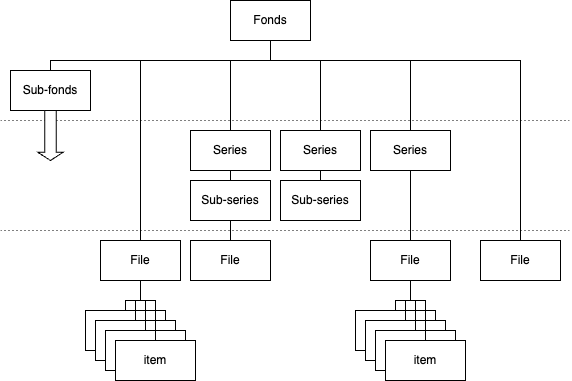
\includegraphics[width=\linewidth]{chapters/3-mdc_model-reactivation_workflow-instruction_template/image/graph03-isadg.png}
    \caption{Graphical representation of the ISAD(G) model’s hierarchical structure.}
    \label{fig:c3-isadg}
\end{figure} 

As outlined in the ISAD(G) text, the hierarchical levels can be described as:
\begin{itemize}
    \item \textit{Fonds}: The whole of the records, regardless of form or medium, organically created and/or accumulated and used by a particular person, family, or corporate body in the course of that creator's activities and functions.
    \item \textit{Series}: Documents arranged in accordance with a filing system or maintained as a unit because they result from the same accumulation or filing process, or the same activity; h
    \item \textit{File}: An organised unit of documents grouped together either for current use by the creator or in the process of archival arrangement, because they relate to the same subject, activity, or transaction. A file is usually the basic unit within a record series.
    \item \textit{Item}: The smallest intellectually indivisible archival unit, e.g., a letter, memorandum, report, photograph, sound recording.
\end{itemize}
The structure is just one perspective of the archival description provided by ISAD(G), the standard also defines 26 descriptive elements to elaborate on the description of each archival entity. However, we have only focused on the hierarchical structure and consider its application for describing artworks. Indeed, this hierarchical structure is highly relevant, as it can serve as a representation of the components and documentation relating to works of art. By adopting the ISAD(G) model, we can consider the artwork as an archival \textit{fonds}, within which all related physical or digital pieces are included. Since live media art often consists of one or more \textit{series} of iterations, these iterations can be viewed as archival \textit{files}. Each archival \textit{file} representing an iteration of the artwork contains all the items that belong to that specific iteration. As illustrated in Figure~\ref{fig:c3-isadg_art}, we can use the ISAD(G) hierarchical model to represent the relationships between the artwork.

\begin{figure}[!h]
    \centering
    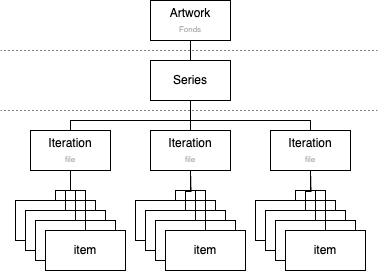
\includegraphics[width=0.7\linewidth]{chapters/3-mdc_model-reactivation_workflow-instruction_template/image/graph03-isadg_art.png}
    \caption{Representation of the artwork as an archive according to the ISAD(G) model’s hierarchical structure.}
    \label{fig:c3-isadg_art}
\end{figure} 

Based on this representation, we could elaborate and formalise the multilevel model developed by the CSC in a more structured way to better represent creative works.

\subsection{Structure}
Figure~\ref{fig:c3-mdc} shows the updated representation of the \textit{Multilevel Dynamic Conservation} (MDC) model. We replaced the diagram structure with a matryoshka-style representation to better illustrate how documentation layers contribute to the artwork's identity.

\begin{figure}[!h]
    \centering
    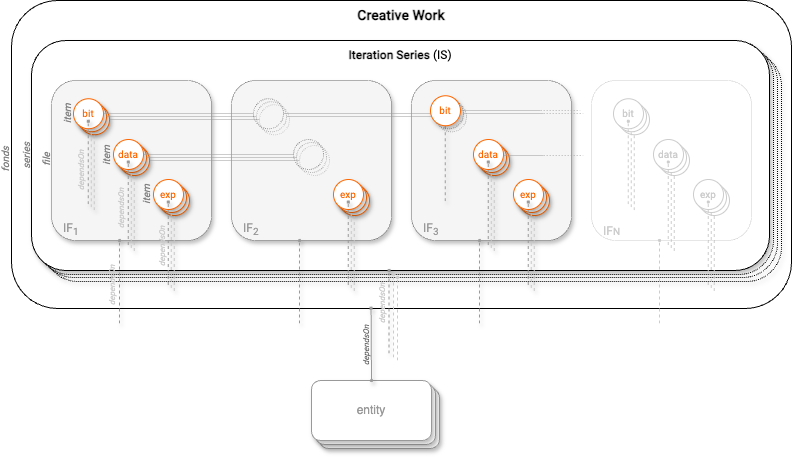
\includegraphics[width=\linewidth]{chapters/3-mdc_model-reactivation_workflow-instruction_template/image/graph03-mdc.png}
    \caption{Graphical representation of the Multilevel Dynamic Conservation (MDC) Model.}
    \label{fig:c3-mdc}
\end{figure} 

The model has three key properties: \textit{multilayering}, \textit{multiple belongingness}, and \textit{dependencies}.\\
Regarding the first property, the model consists of four main levels, arranged hierarchically to move from the general to the specific. The top level represents the \textit{Creative work} itself, which could be an artwork but also an artistic project or artefact. Like a \textit{fonds}, it includes all related items. The \textit{Creative work} consists of an \textit{Iterations Series} (IS), which contains all the manifestations or versions of the work. Typically, a creative work has one IS, but multiple \textit{Iteration Series} can be created in exceptional cases or based on archival needs. Other series types can also be included. For instance, if there are pieces of information unrelated to any specific manifestation but to the creative work as a whole (such as bibliographic references or analysis of an artwork), a dedicated series (like a \textit{Bibliography Series}) can be created. However, only the main IS is mandatory. The IS contains individual iterations called \textit{Iteration Files} (IF). An IF is essentially a container—or folder, in analogy to the ISAD(G) framework—that holds all the items associated with a particular iteration of the work. The lowest level represents the individual items of a work's manifestation (iteration or version). These items are the physical and digital elements that form the artwork, such as the components, instructions, scores or any other documentation that captures the experience of each version. At this level, we can reintroduce the division from the first version of the model. The items within each IF can be grouped into three distinct types:
\begin{itemize}
    \item \textit{Bit}: These are all the physical and digital parts that make up the work, such as hardware, software, installation and performance objects, and fixed-media files (e.g., video or audio components used in the manifestation). 
    \item \textit{Data}: This refers to all the information necessary for realising the work. These elements form the work's instructions, mappings, or scores, particularly regarding how the components (\textit{bit}s) should be linked, used, activated, and arranged in space and time. Examples include operating instructions, musical scores, scripts, technical notes, comments on the work, and high-level descriptions of algorithms and models.
    \item \textit{Experience}: This includes documents that capture the work's experience, such as interviews, audio/video recordings, and usability tests of the original system. It also covers information about the people involved in the realisation of the work (artists, performers, technicians) and their roles. Additionally, any documentation related to the reactivation or preservation of the work (e.g., descriptions of approaches, methodologies, and software used) falls into this category.
\end{itemize}
While these physical and digital elements are collected separately, they should be seen as closely connected and following, even in this case, a hierarchical information structure, as defined by the original multilevel model. Figure~\ref{fig:c3-items} illustrates the artwork's hierarchical structure of \textit{bit}, \textit{data}, and \textit{experience}. 

\begin{figure}[!h]
    \centering
    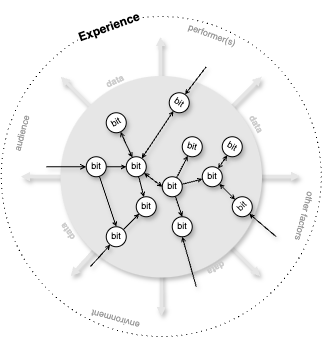
\includegraphics[width=0.7\linewidth]{chapters/3-mdc_model-reactivation_workflow-instruction_template/image/graph03-items.png}
    \caption{The hierarchical structure of bit, data and experience.}
    \label{fig:c3-items}
\end{figure} 

Compared to the previous version of the model, one type of item, the \textit{record}, is no longer necessary. Any modifications to the original artwork are recorded within each \textit{Iteration File}, and the overall changes can be traced by reviewing the \textit{Iteration Series} as a whole.\\
Another essential property of the MDC is the \textit{multiple belongingness}. As we can see in the graphical representation of the model in Figure~\ref{fig:c3-mdc}, \textit{bit} and \textit{data} type items can belong to multiple IFs. If some parts (or even all parts) of the original or previous manifestation are reused in an ongoing reactivation, those will also be registered as elements of the new IF. The \textit{multiple belongingness} of items is an important property of the presented model, which differs from the general structure of the ISAD(G) in which each archival unit (\textit{item}) only belongs to a unique file. The \textit{multiple belongingness} can be applied only to \textit{bit}- or \textit{data}-type items since \textit{experience}-type ones are designed to document the ongoing manifestation. It thus must belong to a unique IF. This property allows the creative work to be represented not as a mere group of delimited records but rather as a process or a dynamic object\footnote{In other words, the experience is the product of the mapping of all \textit{bit} (the \textit{data}) within a specific spatio-temporal context as also shown in Figure~\ref{fig:c3-items}, i.e. it belong to a specific iteration, and can not be the same for other ones}.\\
The same property can be applied at a higher level across different creative works. Items from the \textit{Iteration Series} category (e.g., a software), as well as items from other types of series (e.g., a bibliographic item), can be shared across multiple creative works. Even \textit{experience}-type items can be shared among multiple artworks if the same items document all these multiple artworks. In particular cases, even an entire series can belong to more than one artwork\footnote{Consider the \textit{Reenactments} by the duo 0100101110101101.org mentioned in the previous chapter. Depending on the archival approach, the various presentations (iterations) of the virtualized historical performances can either belong to the specific \textit{Reenactment} by the duo (thus treated as a standalone artwork) or be considered reproductions of the original historical works, performed in a virtual environment, and therefore classified under those original works. The MDC model does not exclude either option, allowing for both interpretations simultaneously.}.\\
The last property of the model is the \textit{dependence} of various levels and items on entities. These dependencies can have different types necessary for applying the model, such as \textit{isOwnedBy}, \textit{isProducedBy}, \textit{isCreatedBy}, \textit{isRealizedBy}, etc. Still, they can also be more specific for exhibitions, such as \textit{isPerformedBy}, \textit{isCuratedBy}, and so on. Entities can also vary depending on the needs, and we can include people, organisations, institutions, companies, etc. Even within the dependency relationships, we can apply \textit{multiple belongingness}, meaning these relationships can be multiple: levels and items can depend on more than one entity, and vice versa, i.e., the same entity can relate to multiple levels or items. This property and \textit{multiple belongingness} allow us to track the artwork's transformation based on the dependency relationships.\\
As a meta-model, the MDC model does not define the metadata structure for digital components or preservation methods for physical ones. Instead, the model states the properties of creative works as a function of their conservation. Informational and practical levels would be defined in constructing an application model. They could refer to existing external standards (e.g., the previously mentioned OAIS reference model for digital items) or requirements of a specific institution.

\section{Reactivation workflow}
Alongside the MDC model, designed to guide the conservation of creative works, we introduce a reactivation workflow to represent the process of reactivating the work with each new iteration.\\
The workflow model was developed in collaboration with the Department of Computational Media and Arts (CMA) at the Hong Kong University of Science and Technology in Guangzhou (HKUST(GZ)), China\footnote{During the PhD research project, a 6-month Visiting Research Program was conducted at HKUST(GZ) with the goal of developing and formalising the reactivation workflow presented here. The 6-month Visiting Research Program was supervised by Assistant Professor Raul Masu.}. The workflow model was initially developed for Digital Musical Instruments (DMIs). While this context differs slightly from live media art, it is still closely related, as it focuses on creating original interfaces for performances, installations, and educational and inclusive applications.\\
In a broad sense, DMIs can be viewed as hardware and software aggregates, consisting of both a controller or gestural interface and a digital sound synthesis method to generate and process sounds in real-time \cite{miranda2006new}. For the development of this workflow, we primarily focused on DMIs developed in the context of the New Interface for Musical Expression (NIME) conference, where new DMIs are presented and implemented in installations and live performances every year\footnote{New Interfaces for Musical Expression website: \url{https://www.nime.org/} (accessed 15/12/2024).}. The conference is based on the usage of new technologies in designing instruments for musical expression, with an increasing focus on audio-visual expression \cite{jensenius2017nime}.\\
However, in recent years, the NIME community has recognised issues surrounding short-term engagement with these instruments, both in terms of reduced artistic use and wasted potential of the devices themselves. A significant problem is that these instruments often fail to be used beyond their initial presentation \cite{mamedes2014nime}. Morreale and McPherson conducted a systematic review of NIME projects \cite{morreale2017nime}, showing that only a small percentage of the devices showcased at the conference have been used in more than one performance. Many research-based DMIs (such as those presented at NIME) often remain as prototypes, abandoned in favour of developing new instruments, compromising both the instruments' mastery and further artistic and expressive experimentation.\\
In response, various studies have examined DMI longevity and sustainability, offering practical guidelines and best practices (e.g., using FLOSS, documenting instruments, employing modular designs, and considering musical outcomes). Despite this, as a recent systematic review \cite{masu2023nime} revealed, among nearly 300 papers published in the 2020–2022 editions of the NIME conference, only 9\% addressed the reuse and repurposing of DMIs, while 67\% introduced new ones\footnote{Notably, this trend does not seem to change: if we consider the proceeding of the NIME 2023, in which only 6 papers deal with the reuse and repurpose of DIM (∼6\% of the 99 papers published).}.\\
In light of this issue and the need for more sustainable solutions, the MDC model has been proposed as a framework for the sustainability and preservation of DMIs. The model was applied in a specific case study: the reactivation of \textit{Soundrise}, an interactive multimedia application for deaf children. A multimedia application is a creative work with challenges similar to live media artworks, such as technology, documentation, interaction, and creative and collaborative processes. However, there is a key difference: for multimedia applications, the evolution of the work is taken for granted, and the final version is the most important (as important as the original in traditional art). Unlike artworks, these applications are not framed within the broad and complex theoretical context of art, and concepts like authenticity and identity are more superficial, often linked to legal matters instead. However, this case study aimed to examine a multimedia application from the perspective of live media art and thus proposing an innovative solution for the sustainability of such creative works. During the application of the MDC model, it became clear that reconstructing an application follows distinct steps, each with specific functions and outcomes. As a result, the study led to the development of a formal workflow to describe the reactivation process.

\subsection{Structure}
\begin{figure}[!h]
    \centering
    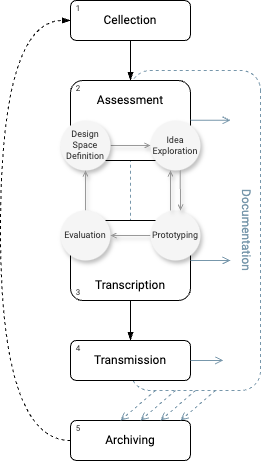
\includegraphics[width=0.7\linewidth]{chapters/3-mdc_model-reactivation_workflow-instruction_template/image/graph03-catta.png}
    \caption{Graphical representation of the CATTA reactivation workflow.}
    \label{fig:c3-catta}
\end{figure} 

Figure~\ref{fig:c3-catta} shows a graphical representation of the reactivation workflow called CATTA. The CATTA workflow consists of five steps, from which its name is derived: \textit{Collection}, \textit{Assessment}, \textit{Transcription}, \textit{Transmission}, and \textit{Archiving}. These five steps aim to ensure consistent reactivation and facilitate future ones. As shown in the graphical representation, the CATTA workflow also includes sub-steps borrowed from the \textit{design process} introduced by Filipe Calegario in \textit{Designing Digital Musical Instrument Using Probatio} \cite{calegario2018designing}. The design process is not exclusively developed for DMIs; it rather functions as a general description comprehending different areas. It is defined by \textit{Design Space definition}, \textit{Idea exploration}, \textit{Prototyping}, and \textit{Evaluation} steps and helps to better nuance the central CATTA’s \textit{Assessment} and \textit{Transcription} steps.\\
As following, we describe the CARIA process steps:
\begin{enumerate}
    \item \textit{Collection}: The first step involves collecting (or acquiring) all of the creative work's components at every stage of its development, from the first manifestation to the latest. In this step, the acquisition includes all physical and digital parts, scores, instructions, and documents that demonstrate the state of the creative work throughout its iterations. The goal is to collect as much information as possible and to have a clear understanding of its dynamics. At this point, pre-acquisition and acquisition steps (as seen in live media art conservation initiatives) can be included, along with the compilation of the \textit{identity report}. If the MDC model is applied, this is where all the artwork’s elements are organised according to its hierarchical and dynamic structure, defining the creative work level (e.g., through the \textit{identity report}) and the \textit{iteration series} by completing the iteration files and classifying the elements as \textit{bit}, \textit{data}, or \textit{experience}.
    \item \textit{Assessment}: This step involves evaluating any issues, problems, vulnerabilities, and the potential of the previous versions of the work. Condition reports can be created (if not already available), and depending on preservation choices, assessments can be done at the level of the creative work, individual iterations, or both. However, this evaluation does not just focus on past iterations but mainly looks forward to future ones. The CATTA process is used when creative works need to be reactivated, so assessments must not only address weaknesses but also plan for the upcoming reactivation, thus finding the best conditions for the work to continue to exist. Therefore, new parameters for reactivation are necessary to consider, and they depend on various factors like space, the event, performers, etc. In other words, we are now looking at the variables that enable the necessary negotiation among the different ecosystems—essential for conserving the creative work, or more precisely, for ensuring its survival during this reactivation and the next one.\\
    At this point, we include the design process's sub-steps of \textit{Design Space definition} and \textit{Idea exploration}. The \textit{Design Space definition} is ``\textit{related to understanding the concept [of the reactivation], such as the stakeholders, the scenarios, the common knowledge of the area: understanding the user’s interaction and context of use; and defining restrictions that define the designing space of the project}'' \cite{calegario2018designing}. The \textit{Design Space} ``\textit{constraints design possibilities along some dimensions, while leaving others open for creative exploration}" \cite{beaudouin2003prototyping}. In practice, the \textit{Design Space} is defined by the collected elements and the context in which the work will be presented. This sub-step involves not only following the artist's instructions (intentions and constraints) and adapting them to a new context or evaluating the \textit{bit}s (physical and digital components) that may be missing or malfunctioning. It also involves considering the circumstances of the reactivation, such as the event, purpose, and the economic conditions underlying it.\\
    Once these boundaries are defined, the next sub-step is \textit{Idea exploration}, where potential development paths are explored. In this sub-step, we try to expand the \textit{Design Space}, especially in very constrained cases—like when an artwork is site-specific or tied to a particular historical moment. We may also explore technology migration, emulation, or even complete reinterpretations of the work. During this sub-step, a decision-making tool, such as DOCAM’s \textit{Decision Tree}, can be applied to evaluate development paths.\\
    The \textit{Design space definition} and \textit{Idea exploration} sub-steps defined in \cite{calegario2018designing} offer a structured method for determining the creative work’s \textit{changeability}.
    \item \textit{Transcription}: After identifying possible development paths and thus the \textit{changeability}, the \textit{transcription} step aims to create ``prototypes'' of the reactivation, evaluate their effectiveness, and finally produce the concrete reactivation of the creative work.\\
    This step includes two sub-steps: \textit{Prototyping} and \textit{Evaluation}. In \textit{Prototyping}, the reactivation ideas are implemented, focusing on practical and functional aspects. Here, the collected \textit{bit}s are assembled according to the instructions (\textit{data}). New \textit{bit}s may be introduced depending on the development path, so new assembly criteria and instructions must be developed. The prototyping process is not done in one go; it passes through different stages and levels of fidelity, which are evaluated during the \textit{Evaluation} sub-step. \textit{Prototyping} can be experimental, testing different development paths, or exploratory, overlapping with the previous \textit{Idea Exploration} step. Prototypes range from \textit{low-fidelity}—where representations are simple, usually on paper, with limited details and focused on specific aspects (initial prototype)—to \textit{high-fidelity}–where the development path is applied concretely with many details (working prototype). \\
    Each prototype requires evaluation to either continue and improve the prototyping process or to reassess the documentation, returning to the \textit{Assessment}'s \textit{Design Space} definition sub-step to redefine the approach.\\
    During the \textit{transcription} phase, all the activities needed to make the creative work accessible to the public should be considered and developed. They include setting up the artwork in relation to other works, promoting it, creating catalogues, and providing general information.
    \item \textit{Transmission}: After the transcription step, the artwork should be functionally reactivated, meaning it is ``transmitted'' to the audience so they can experience it. The transmission involves the performer(s) and the audience interacting with the work, generating the experience of that specific creative work.
    \item \textit{Archiving}: The final step is archiving the documentation produced during reactivation. This step is crucial for conservation. All the other steps generate a large amount of documentation: condition reports and other evaluations from the \textit{assessment}; all prototypes and evaluations from the \textit{transcription} step (which often produces the most information); and documentation about the setup and, most importantly, the experience of the artwork during the \textit{transmission}. Only by archiving this documentation can future reactivations take place, ensuring the conservation of the creative work.
\end{enumerate}
The separation of steps in the CATTA process is not rigid; the steps do not follow in a strictly discrete order but rather overlap and intertwine. Although the \textit{assessment} step is supposed to begin after all elements of the artwork are collected, these two steps can also occur simultaneously, as each piece of the work can be assessed during the collection phase. Additionally, the \textit{assessment} and \textit{transcription} steps interact closely. During the \textit{transcription}, it is often necessary to return to the \textit{assessment} phase (as described in the design processes’ sub-steps). The \textit{transcription} step can also overlap with the \textit{transmission} step. For example, issues that arise during setup or installation, or new unforeseen behaviours observed when the artwork interacts with the audience, may require reevaluation and adjustments, causing a return to the \textit{transcription} (or even the \textit{assessment}) step. The \textit{archiving} step is the most evident case of overlap, as it should ideally take place alongside the other steps, which are generating documentation, rather than only after all the other steps are completed. Therefore, the steps are more or less simultaneous, and their incremental order is not purely sequential or time-based but rather based on dependencies. For instance, we can conduct an \textit{assessment} if we have some collected documents (even just one), move to \textit{transcription} based on an \textit{assessment}, proceed with \textit{transmission} if we have a functioning work, and finally, \textit{archiving} can only happen if documentation has been produced in the other steps.

\section{Modular Instruction Template (MIF) and Baalman Visual Language (BVL)}
Finally, we introduce the last system: the \textit{Modular Instruction Framework} (MIF). This system was developed to guide the documentation of the technical information needed to reactivate the artwork—i.e., the \textit{data} level in the MDC model. Referring back to the MDC model’s graphical representation and Figure \ref{fig:c3-items}, which illustrates the hierarchical structure of items, we can see that the \textit{data} level is crucial. The \textit{data} connects all the \textit{bit}s to each other (at the lowest level) and to the \textit{experience} (at the highest level). In simpler terms, the \textit{data} level is like the brain of the work and a key element in its conservation. It consists of the information that defines how all the elements relate to each other across different dimensions (spatial, temporal, processual, gestural, etc.). The \textit{data} largely contributes to determining the work’s identity, meaning that the same group of \textit{bit}s can create two entirely different \textit{experiences} depending on how they are mapped.\\
While we can easily identify a \textit{bit} or a piece of \textit{experience} (like a computer, software, audiovisual file, or photo), defining \textit{data} is less straightforward. How do we concretely describe it? Is it a diagram, a set of instructions, a score, or a combination of these things? Can it be seen as a multimedia file, a fixed digital text, or something on paper? Do we need to follow specific notational systems or standards?\\
In this section, we will clarify the concept of \textit{data} and offer practical solutions for compiling this level.\\
The \textit{data} level contains all the information on how to set up and run the work, including instructions, musical scores, high-level descriptions of algorithms, and so on. In other words, it includes information on \textit{bit}s and their interaction, including the interaction with external agents such as the environment, performers, audiences, and other factors. Unlike the usual comparison with a score, here we introduce the term \textit{mapping} to group all these types of ``information'' —a term typically used in the field of interaction design. Mapping is essential for describing the artwork because it captures the core elements ``\textit{where the artist expresses themselves}'' \cite{baalman2022composing}. As Marije Baalman states, ``\textit{The question of mapping is central to creating artistic meaning in interactive, digital art}'' \cite{baalman2022composing}. Mapping can be seen as the invisible part \cite{delahunta2001invisibility} of interactive work, the element that connects gestures (of any kind, from a controlled action by a performer to an uncontrolled action by a non-human actor, i.e., any physical phenomenon that changes over time) with specific outputs (lights, sounds, videos, heat, robot movements, fan-generated wind, vibrations, etc.). Here, however, we use the term mapping more broadly, not only to describe high-level experiences but also the communication between hardware and software components, defining it as the ``\textit{matching of one element of a set with another element in the same set or in a different set}'' \cite{winkler2001composing}.\\
For example, in the case study \textit{Il caos delle sfere} (Appendix~\ref{ax:b-hybrid_reactivation_il_caos_delle_sfere}), we can identify multiple levels of mapping description, starting from a conceptual level where the pinball game (gestures) is connected to the notes played by the Disklavier (the sound output). At a lower level, the pinball machine's sensors are processed by a specific PCB that converts signals and sends them to a computer via a 25-pin parallel port; the computer then converts the signals through dedicated software and sends MIDI notes via a MIDI connection to a Disklavier, which ultimately transforms the MIDI notes into mechanical movements that strike the piano keys. This description could go further, detailing the components and their communication in the PCB construction or the functionality of the dedicated software. The levels of detail in mapping descriptions vary, functioning like a matryoshka doll. The more specific the details, the more precise the reconstruction of the artwork, leaving less room for reinterpretation and slowing down the dynamic nature of the artwork's identity.\\
Mapping descriptions are usually documented on paper or in static digital files using diagrams, representations, or pseudo-descriptions. However, there are no standardised formats or notation languages for these descriptions.\\
An example of mapping notation language that is not standardised but broadly shared, even with more or less divergences, can be found in live electronic music scores. Case studies on live electronic music carried out in this research project aimed to study score development and performance instruction definitions (explored further in Appendix~\ref{ax:c-the_score_in_live_electronics_music}). The section~\ref{sec:ac-score-section} of Appendix~\ref{ax:c-the_score_in_live_electronics_music} analyses the structures of the six principal scores studied and used for performance. Although there are differences between the score structures, certain fundamental elements recur, especially for the electronic part. Those elements are:
\begin{itemize}
    \item \textit{Live Electronics instruments list};
    \item \textit{Disposition or Stage plan} (graphic representation of the arrangement of acoustic and electroacoustic instruments and performers);
    \item \textit{Processing and Parameters definition} (explanation of processing and parameters);
    \item \textit{Performance instructions} (usually textual, with graphic representations of gestures or score notations);
    \item \textit{Schemas and Routing};
    \item \textit{Score}.
\end{itemize}
While the \textit{Electronic instrument list} represents a list of the \textit{bit}s, all other parts represent the mapping, each from a different perspective or level. There is spatial mapping (\textit{Disposition and Stage Plan}), where \textit{bit}s are mapped into a physical space; temporal mapping, represented not only by the \textit{score} but also by the \textit{Performance Instructions}, which define the performers' gestures in relation to the \textit{bit}s; and other types of mapping that detail the relationships between electroacoustic instruments, inter-process relationships, and signal processing behaviour (represented by \textit{Schemas and Routing}) and \textit{Processing and Parameters}). No standard notation exists for these mappings, though informal solutions are commonly used in live electronic music scores. Standard musical notation is often supplemented with original symbols and explanations in varying amounts of text (\textit{Performance instructions}). Spatial arrangements are represented by scaled-down spaces, where acoustic and electroacoustic instruments are stylized. Similarly, the exact placement of microphones on instruments can be shown (e.g., in the \textit{Cantare con Silenzio}’s score). Representation forms borrowed from electrical circuits, schematics, and diagrams are often used to describe \textit{Schemas and Routing} which represent signal processing mappings.\\
Although these representation methods originate from electronic music, they have also been adopted and used in other fields (e.g., dance, video art, and multimedia installations). With the developing interest in live media art (especially in the conservation field), new proposal strategies and representation methods for mapping (or score) compliance have been proposed with different levels of detail. One of the most interesting recent proposals is the Visual Language introduced by Marija Balmaan in \textit{Composing Interaction} \cite{baalman2022composing}, a notation system for describing performance and digital art mappings.\\
\begin{quote}
    “The visual language can be used on various different levels: to describe concepts (who performs which gesture, what effects the gesture) and spatial layouts, to illustrate the flow of actions, the different signals, or to describe the physical elements and their connections, and so on. This can be a broad description or a detailed documentation of how a particular filter is implemented. You can use the language to zoom in on detail and zoom out to get an overview of you project” \cite{baalman2022composing}.
\end{quote}
The visual language proposed by Baalman–which we will henceforth refer to by the acronym BVL (\textit{Baalman Visual Language})– is very similar to the block diagrams used in electronic music scores. However, it is an attempt to formalise this type of notation for use in multimedia arts in general. The language is based on simple symbols and blocks representing concepts, elements, and connections. These can be expanded with names and descriptions. The language has three main levels of definition:
\begin{itemize}
    \item \textit{Conceptual Level}: This describes what happens in the artwork, including the gestures involved, the outputs produced, and the spatial layout of the interaction. It answers the questions ``Who (the actor [, e.g., performer, audience, etc.]), what (specific parts/elements of the actor), the action or gesture, how the gesture is performed, and the effect of the action (what happens in the output medium).'' The visual language here consists of a series of elements (actor, physical element, concept clarification, action, and effect) that can be linked together in a flowchart or spatial diagram.
    \item \textit{Physical Implementation level}: This describes what happens between the gesture and the output medium, detailing which physical and digital \textit{bit}s are used and how they are connected. At this level, the visual language consists of blocks representing the different \textit{bit}s, connected by arrows that show how they interact.
    \item \textit{Process Level}: This explains how the data generated by gestures is processed to produce the output. It describes how various processes communicate and, using sub-levels, shows how individual processes occur and how data streams are handled and processed. This level mainly uses squares connected by arrows. The squares and connections can be expanded with verbal descriptions to indicate specific processes and data streams.
\end{itemize}
\begin{figure}[!h]
    \centering
    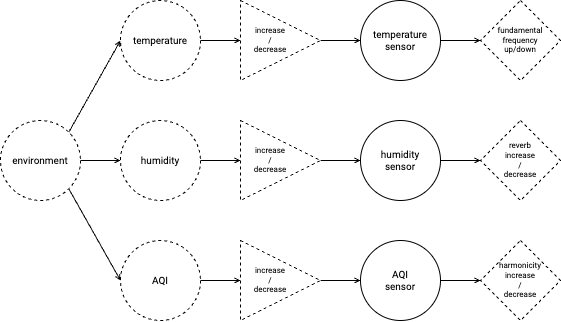
\includegraphics[width=0.7\linewidth]{chapters/3-mdc_model-reactivation_workflow-instruction_template/image/graph03-BVLconcept.png}
    \caption{Description of the installation through Baalman’s Visual Language - Conceptual level.}
    \label{fig:c3-BVLconceptual}
\end{figure} 
\begin{figure}[!h]
    \centering
    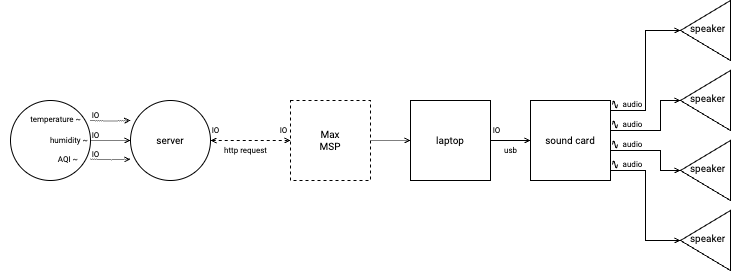
\includegraphics[width=0.7\linewidth]{chapters/3-mdc_model-reactivation_workflow-instruction_template/image/graph03-BVLphysical.png}
    \caption{Description of the installation through Baalman’s Visual Language - Physical implementation level.}
    \label{fig:c3-BVLphysical}
\end{figure} 
\begin{figure}[!h]
    \centering
    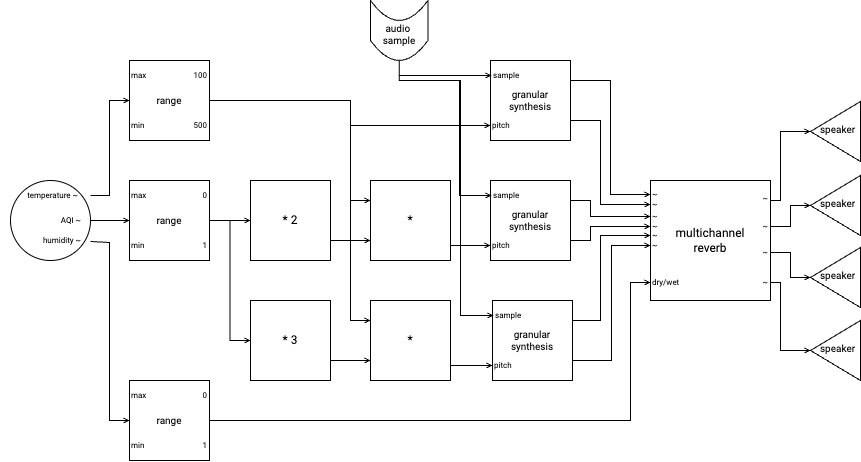
\includegraphics[width=0.7\linewidth]{chapters/3-mdc_model-reactivation_workflow-instruction_template/image/graph03-BVLprocess.png}
    \caption{Description of the installation through Baalman’s Visual Language - Process level (Highest level of representation).}
    \label{fig:c3-BVLprocess}
\end{figure} 
Figures~\ref{fig:c3-BVLconceptual}, ~\ref{fig:c3-BVLphysical} and ~\ref{fig:c3-BVLprocess} are some examples of how this visual language was applied in a creative case study aimed at studying the application of live media art installation documentation\footnote{This case study will not be explored in depth through a separate chapter unlike the other studies mentioned so far. We have chosen to omit it for the brevity and simplicity of the study, even though it was useful for exploring the application of BVL.}. In short, the study involves creating and documenting a sound installation in which data from a public air quality monitoring station controls the parameters of sound played in a room through four speakers.\\
Figure~\ref{fig:c3-BVLconceptual} shows the \textit{Conceptual level}, Figure~\ref{fig:c3-BVLphysical} shows the \textit{Physical implementation level}, and Figure~\ref{fig:c3-BVLprocess} shows the \textit{Process level} (shown at a high level, meaning you can zoom in and add more detail to the process).\\
This BVL is very useful, mainly because it remains flexible, allowing for creating new blocks and connections as needed. Its usage is also very versatile and fits well with the meta-model described earlier, as it can be applied to different levels of complexity. One can even use the visual language to hand-draw a mapping on paper, without needing any specific tools. Indeed, we will apply BVL in this text to represent the mappings of the case studies. In the next chapter, we will adapt the BVL to be used with Diagram.net, an online, free, and cross-platform system that can be used to draw diagrams.\\
However, while this language is adequate for describing process mappings, it does not address other crucial types of mappings, such as \textit{Temporal mapping} (e.g., what happens during a performance and when specific actions occur) and \textit{Spatial mapping} (e.g., the relationship between \textit{bit}s and physical space, such as a stage or a room). The stage plans used in live electronic music scores for \textit{Spatial mapping} remain highly effective, while defining \textit{Temporal mapping} is more complex. Generally, we must rely on something other than the musical notation system. As a result, this mapping type remains more open, varying from case to case\footnote{It is important to note that temporal mapping is especially useful in performance contexts. For example, in interactive installations, there is usually no need to guide the timing of interactions between gestures and the artwork made by the actors (such as the audience, the environment, or other factors). In interactive installations, a set of gestures and their relationships to the artwork are typically defined before implementation, but without specifying the order in which these gestures occur. The gestures appear randomly, depending on how actors interact with the piece.}. We can use graphical representations (either stylised or sequential, such as in the case study of Michele Sambin’s \textit{videoloop} in Appendix~\ref{ax:a-michele_sambin_videoloop}), written descriptions, custom notational systems (which would require a legend and preliminary definitions), multimedia files, or specific tools\footnote{Some tools are those developed for motion notation, especially in dance, by the \textit{Motion Bank} project at the University of Applied Sciences Frankfurt \url{https://motionbank.org/} (accessed 10/010/2024). Another interesting project is that one proposed by University of Udine’s Camera Ottica Laboratory for the classification of moving image \cite{costronuovo2024toward}.}.\\
Based on electronic music scores and BVL, we can define the \textit{Modular Instruction Framework} (MIF). The MIF is a template composed of multiple modules, each serving a specific informative function for compiling instructions to reactivate a creative work. Its modular design provides greater freedom when completing each module–none of the forms are mandatory–and, most importantly, allows them to be updated and changed separately over the course of the work’s various iterations.
\begin{itemize}
    \item \textit{Bit lists and specifications}: A textual document containing a list of all the bits (components) used in the artwork, with possible definitions and specifications. Multiple lists can be drawn up according to specific criteria (like electronic music scores, where you might have lists for acoustic instruments, electroacoustic instruments, and sound processing tools).
    \item \textit{Concepts and Notes}: A textual file that contains information about the artwork's identity, with various notes about the work itself or the instructions (e.g., who wrote the instructions and how they were written).
    \item \textit{Mappings}: Multiple documentation with all the mappings defined from different perspectives. This section can include the following sub-parts:
    \begin{itemize}
        \item \textit{Legend and Note}: Introduction and definition of the visual language used to describe the mappings.
        \item \textit{Parameters}: Any specific parameters related to the \textit{bit}s.
        \item \textit{Concept}: The conceptual level of the BVL, which can be expanded with additional text.
        \item \textit{Physical}: The physical implementation level of the BVL, which is also expandable by text.
        \item \textit{Process}: The process level of the BVL, again with extra explanation.
        \item \textit{Spatial}: The arrangement of \textit{bit}s and actors in space, which can be represented through a stage plan (or, more generally, a space plan).
        \item \textit{Temporal}: The definition of gesture-to-artwork relationships in the time domain. These mappings involve open graphical representations that should be explained in the Legend and Note section.
    \end{itemize}
    \item \textit{Graphical Information}: Multiple documents with text and images or diagrams that provide more detailed explanations of specific instructions (especially regarding the visual appearance of the artwork).
\end{itemize}

Examples of the MIF application can be seen in Appendices~\ref{ax:a-michele_sambin_videoloop}, ~\ref{ax:b-hybrid_reactivation_il_caos_delle_sfere}, \ref{ax:c-the_score_in_live_electronics_music}, and \ref{ax:d-sustainability_and_longevity_of_nimes}.  

\section{Summary}
The systems introduced in this chapter are closely based on the new conservation paradigms and serve as a synthesis of them. They allow for a practical visualisation of these paradigms and, therefore, the entire state of the art.
The MDC model, as a meta-model, does not define a specific conservation model but rather outlines the properties of creative works in relation to their conservation, focusing on the relationships between the various components and the quality of becoming. We define \textit{bit}s, \textit{data}, and \textit{experience} within their hierarchical structure. Still, we do not define their essence (except as an example)—whether digital or physical documentation, software or hardware components, etc. Thus, although we have seen that documentation plays a central role in conservation, the MDC model is not exclusively intended for it. This flexibility is why the MDC distinguishes it from the other models we have discussed so far and also why we intended it as a meta-model. As mentioned several times throughout this text, the artwork's materiality may be secondary to the documentation, but eliminating it is not always possible. Depending on the creative work or the choices made by an institution or one or more conservators, material elements can become part of the conservation process and thus be included within the MDC model. Therefore, the meta prefix should be seen as a way of surpassing a defined model but still providing a framework for creating and describing the conservation of live media art.\\
We can highlight the multilayered and dynamic qualities to compare the MDC model with the state-of-the-art and conservation paradigms. Starting with the multilayered aspect, we saw that it is defined from the first version of the model (based on the preservation framework for scientific data used in computer science) and the analogy of creative works as a multi-typological archive, alongside the use of ISAD(G). We have already seen something very similar in the documentation model developed by the DOCAM research alliance. The \textit{DOCAM Documentation Model} is based on and extends the \textit{Functional Requirements for Bibliographic Records} (1998) \cite{plassard1998functional} of the IFLA Study Group. The extension adds the \textit{component} sublevel, which is ``\textit{at the very heart of the changes affecting most media artworks}''\footnote{For more details on the \textit{DOCAM Documentation Model}, please refer to Chapter~\ref{ch:1-state_of_the_art} or visit the DOCAM research aliance's website at the following link: \url{https://www.docam.ca/en/documentation-model.html} (last accessed 16/12/2024). Further information about the \textit{Functional Requirements for Bibliographic Records} (1998) can be found at the following link: \url{https://repository.ifla.org/items/54925d49-b08d-4aeb-807c-1b509ec40b55} (last accessed 16/12/2024).} The MDC model can, in turn, be seen as an extension of the \textit{DOCAM Documentation Model}. Figure~\ref{fig:c3-mdc-docam} shows a comparison between the \textit{DOCAM Documentation Model} and the MDC multilayering properties.

\begin{figure}[!h]
    \centering
    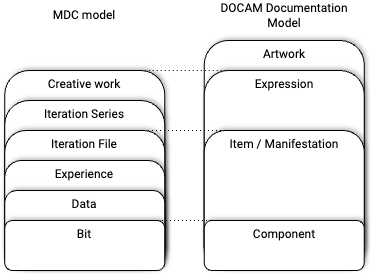
\includegraphics[width=0.5\linewidth]{chapters/3-mdc_model-reactivation_workflow-instruction_template/image/graph03-mdc-docam.png}
    \caption{Comparison between the \textit{DOCAM Documentation Model} and the MDC Model as extension in the multilayering property}
    \label{fig:c3-mdc-docam}
\end{figure}

Regarding the model’s dynamic quality, we see that the \textit{Iteration Series} (IS) tracks the artwork’s biography, and the property of \textit{multiple belongingness} allows for a fluid tracking of transformations and, therefore, identity. Although the dynamic character of the model follows examples from previous models, especially the \textit{Documentation Model for Time-based Media Art} by Joanna Phillips \cite{phillips2015reporting}, it goes beyond them, particularly in its relationship with identity. This model aims to surpass the \textit{allographic} and \textit{two-stage} concept, not considering the relationship from identity to manifestation (dynamic authenticity) as one-directional but bidirectional (as shown in Figure~\ref{fig:c2-authenticity}), or rather, as expressed by the model itself, as a property. For this reason, we chose a matryoshka structure. In the MDC model, the manifestations within the IS are also within the \textit{Creative Work}. Therefore, the series of manifestations are properties of the \textit{Creative Work} and thus define its identity.\\
The property of \textit{dependency} in the MDC model is also significant, especially in relation to the \textit{ecological turn} discussed in the previous chapter. The dependency of levels and items on entities allows us to track the transformation of the artwork and view it in relation to the actors (\textit{actants}) responsible for that transformation. By visualising the dependencies of the artwork across various levels, we can reconstruct the dynamic ecology of its existence and, therefore, the interaction of the different ecosystems at play across the iterations.\\
If we compare the CATTA reactivation workflow with the MDC model, the former is essentially an extension of conservation, representing the loop between documentation and reactivation. Figure~\ref{fig:c3-mdc-catta} shows the relationship between the two systems.

\begin{figure}[!h]
    \centering
    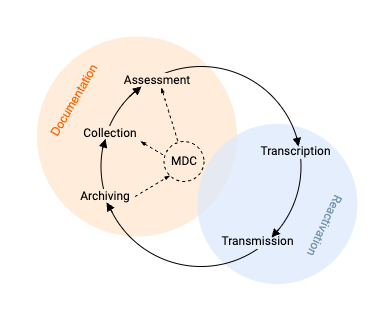
\includegraphics[width=0.8\linewidth]{chapters/3-mdc_model-reactivation_workflow-instruction_template/image/graph03-mdc-catta.png}
    \caption{The CATTA process extends the loop between documentation and reactivation discussed in the previous chapter. In this context, the MDC model serves as a tool used at both the beginning and end of each iteration, facilitating the archiving, collection, and assessment of documentation related to the artwork.}
    \label{fig:c3-mdc-catta}
\end{figure}

As summarised by the figure, the \textit{Collection}, \textit{Assessment} and \textit{Archiving} deal with the documentation and relate to the MDC model. At the same time, \textit{Transcription} and \textit{Transmission} are the two actions that occur during the reactivation. In this case, the MDC model is an instrument for archiving and then collecting and assessing the documentation for each reactivation.\\
Finally, the last system we introduced is the \textit{Modular Instruction Framework} (MIF), a set of optional modules used to create technical instructions for a creative work. The MIF is the result of combining the electronic music scores analysed in Appendix~\ref{ax:c-the_score_in_live_electronics_music} with Baalman’s Visual Language (BVL).\\
Regarding the MIF, it’s important to note that compiling comprehensive instructions can be time-consuming, depending on how complex the work is and how much detail is needed. As mentioned earlier, the \textit{data} level is crucial for conservation. The more detailed this level becomes, the more the artwork’s identity is fixed—which, as discussed in the previous chapter, may not always be necessary for the work itself or for the artists and conservators involved.


